\section{Process definition} 



Framed in the context of an intracellular infection which ultimately causes the host cell to burst, our chosen version of the birth-death catastrophe model is constructed in the following way. $\xt$, is a stochastic process of discrete state-space, evaluated in continuous time. It satisfies the Markov property with transition probabilities dependent only on its current state:
\begin{align*}
\pr{\xx_{t+\Delta t} - \xt = 1} &= \beta \xt \cdot \delt&&\text{(birth)}\\
\pr{\xx_{t+\Delta t} - \xt = -1} &= \mu \xt  \cdot \delt&&\text{(death)}\\
\pr{\xx_{t+\Delta t} - \xt = 0} &=1 -  (\beta+\mu+\delta) \xt  \cdot \delt&&\text{(no event)}\\
\pr{\xx_{t+\Delta t} = H} &=\delta \xt  \cdot \delt&&\text{(catastrophe)}
\end{align*}
The count, $\xt$, is a number of replicative units which in our case representing infectious particles. With rate $\beta$, a given one of these units will undergo division, a birth event; with rate $\mu$, a death event. And with rate $\delta$, a given particle will trigger the catastrophe event. With this staged as rupture of the infected macrophage, all $\xt$ of the virions or bacteria are released into the extracellular matrix. 

In a duration, $\delt$, the probability of a birth occurring is $\beta \delt \cdot \xt$; likelihood of a single unit dividing, multiplied by the number of units, $\xt$. The model is evaluated in the limit, $\delt \to 0$. This is why the above transition probabilities account for only the occurrence of single events. The likelihood that two or more transitions occur in $\delt$ time is proportional to $o(\delt)$, and thus will vanish in the limit.

\begin{figure}[H]
\centering
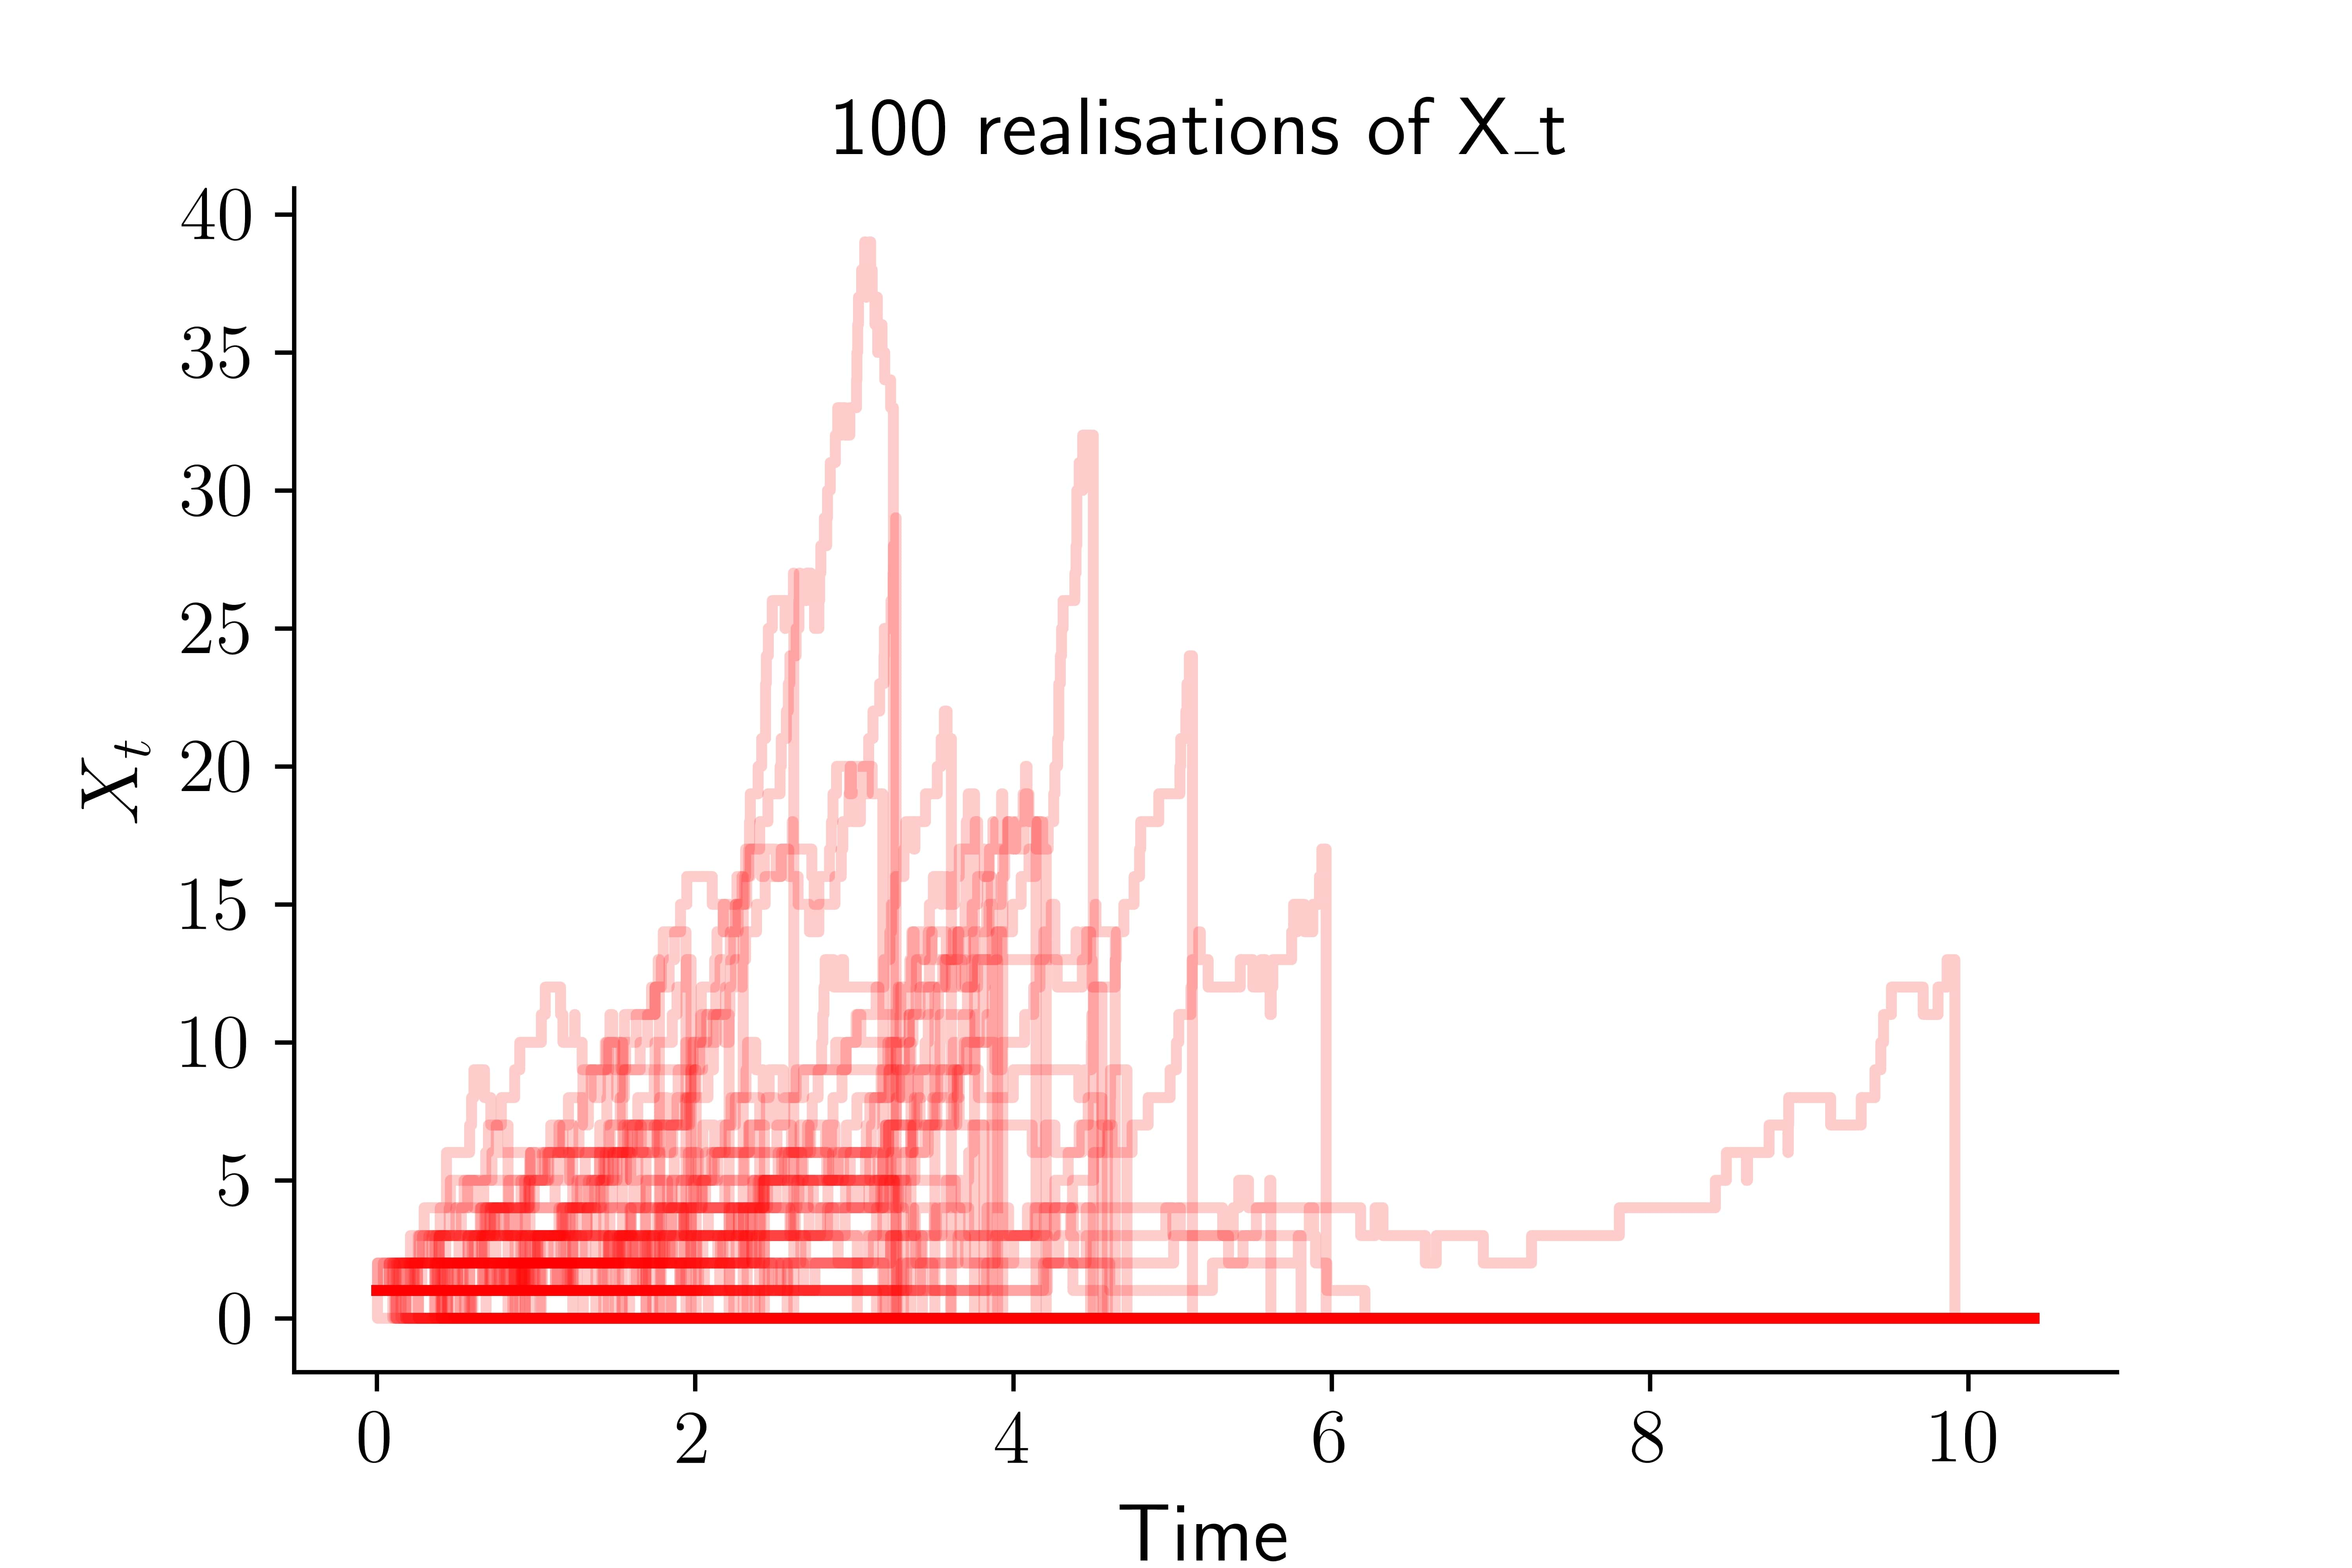
\includegraphics[width = 0.7\textwidth]{figures/IMG_ch4/BDRsimulations.jpg}
\caption{100 realisations of $\xt$ generated using the Gillespie algorithm. $\beta = 1$, $\mu = 0$, $\delta = 0.1$. }
\label{BDRsims}
\end{figure}


\subsection*{Choice of rupture state}


An alternative definition lists the ``catastrophe state'' as 0 instead of a $H$. And it would make some intuitive sense to arrange the process like this. After all, following rupture of an infected cell, there are subsequently 0 replicative units within it. But then, it also no longer exists. Ultimately, whether we ascribe the catastrophe state to 0 or $H$ is of no material significance to the dynamics. That is to say, the burst time and sizes observed are unchanged. But there is a distinction created in some of the formulas. These will be mentioned as we continue, but for our purposes, the catastrophe transition will be taken to the isolated state $H$. \par



\subsection*{Post catastrophe count}

For the context we are considering in which the catastrophe signifies the rupture of an infected cell, following this release, some count of infections units will enter the extracellular medium. This post rupture count, assuming no further dynamics, will be fixed by the final value of $\xt$ prior to catastrophe, and it will remain at that value for future time. We will refer to this post rupture count as $\wt$, itself a stochastic process. $\wt = 0$ for $t\leq\tau$, and $\wt = \xx_\tau$ thereafter for $t> \tau$. ($\tau$ being the time of cell rupture).\par
$\wt$ is included in the above definition as follows to describe the full stochastic process, ($\xt$, $\wt$).
\begin{align*}
\pr{\Delta \xt = 1, \Delta \wt = 0} &= \beta \xt \cdot \delt&&\text{(birth)}\\
\pr{\Delta \xt = -1, \Delta \wt = 0} &= \mu \xt  \cdot \delt&&\text{(death)}\\
\pr{\Delta \xt = 0, \Delta \wt = 0} &=1 -  (\beta+\mu+\delta) \xt  \cdot \delt&&\text{(no event)}\\
\pr{\xx_{t+\Delta t} = H, \ww_{t+\Delta t} = \xx_t} &=\delta \xt  \cdot \delt&&\text{(catastrophe)}
\end{align*}
(Using shorthand, $\Delta \xt = \xx_{t+\Delta t}  -  \xt$).


\begin{figure}[H]
\centering
\title{$\wt$}
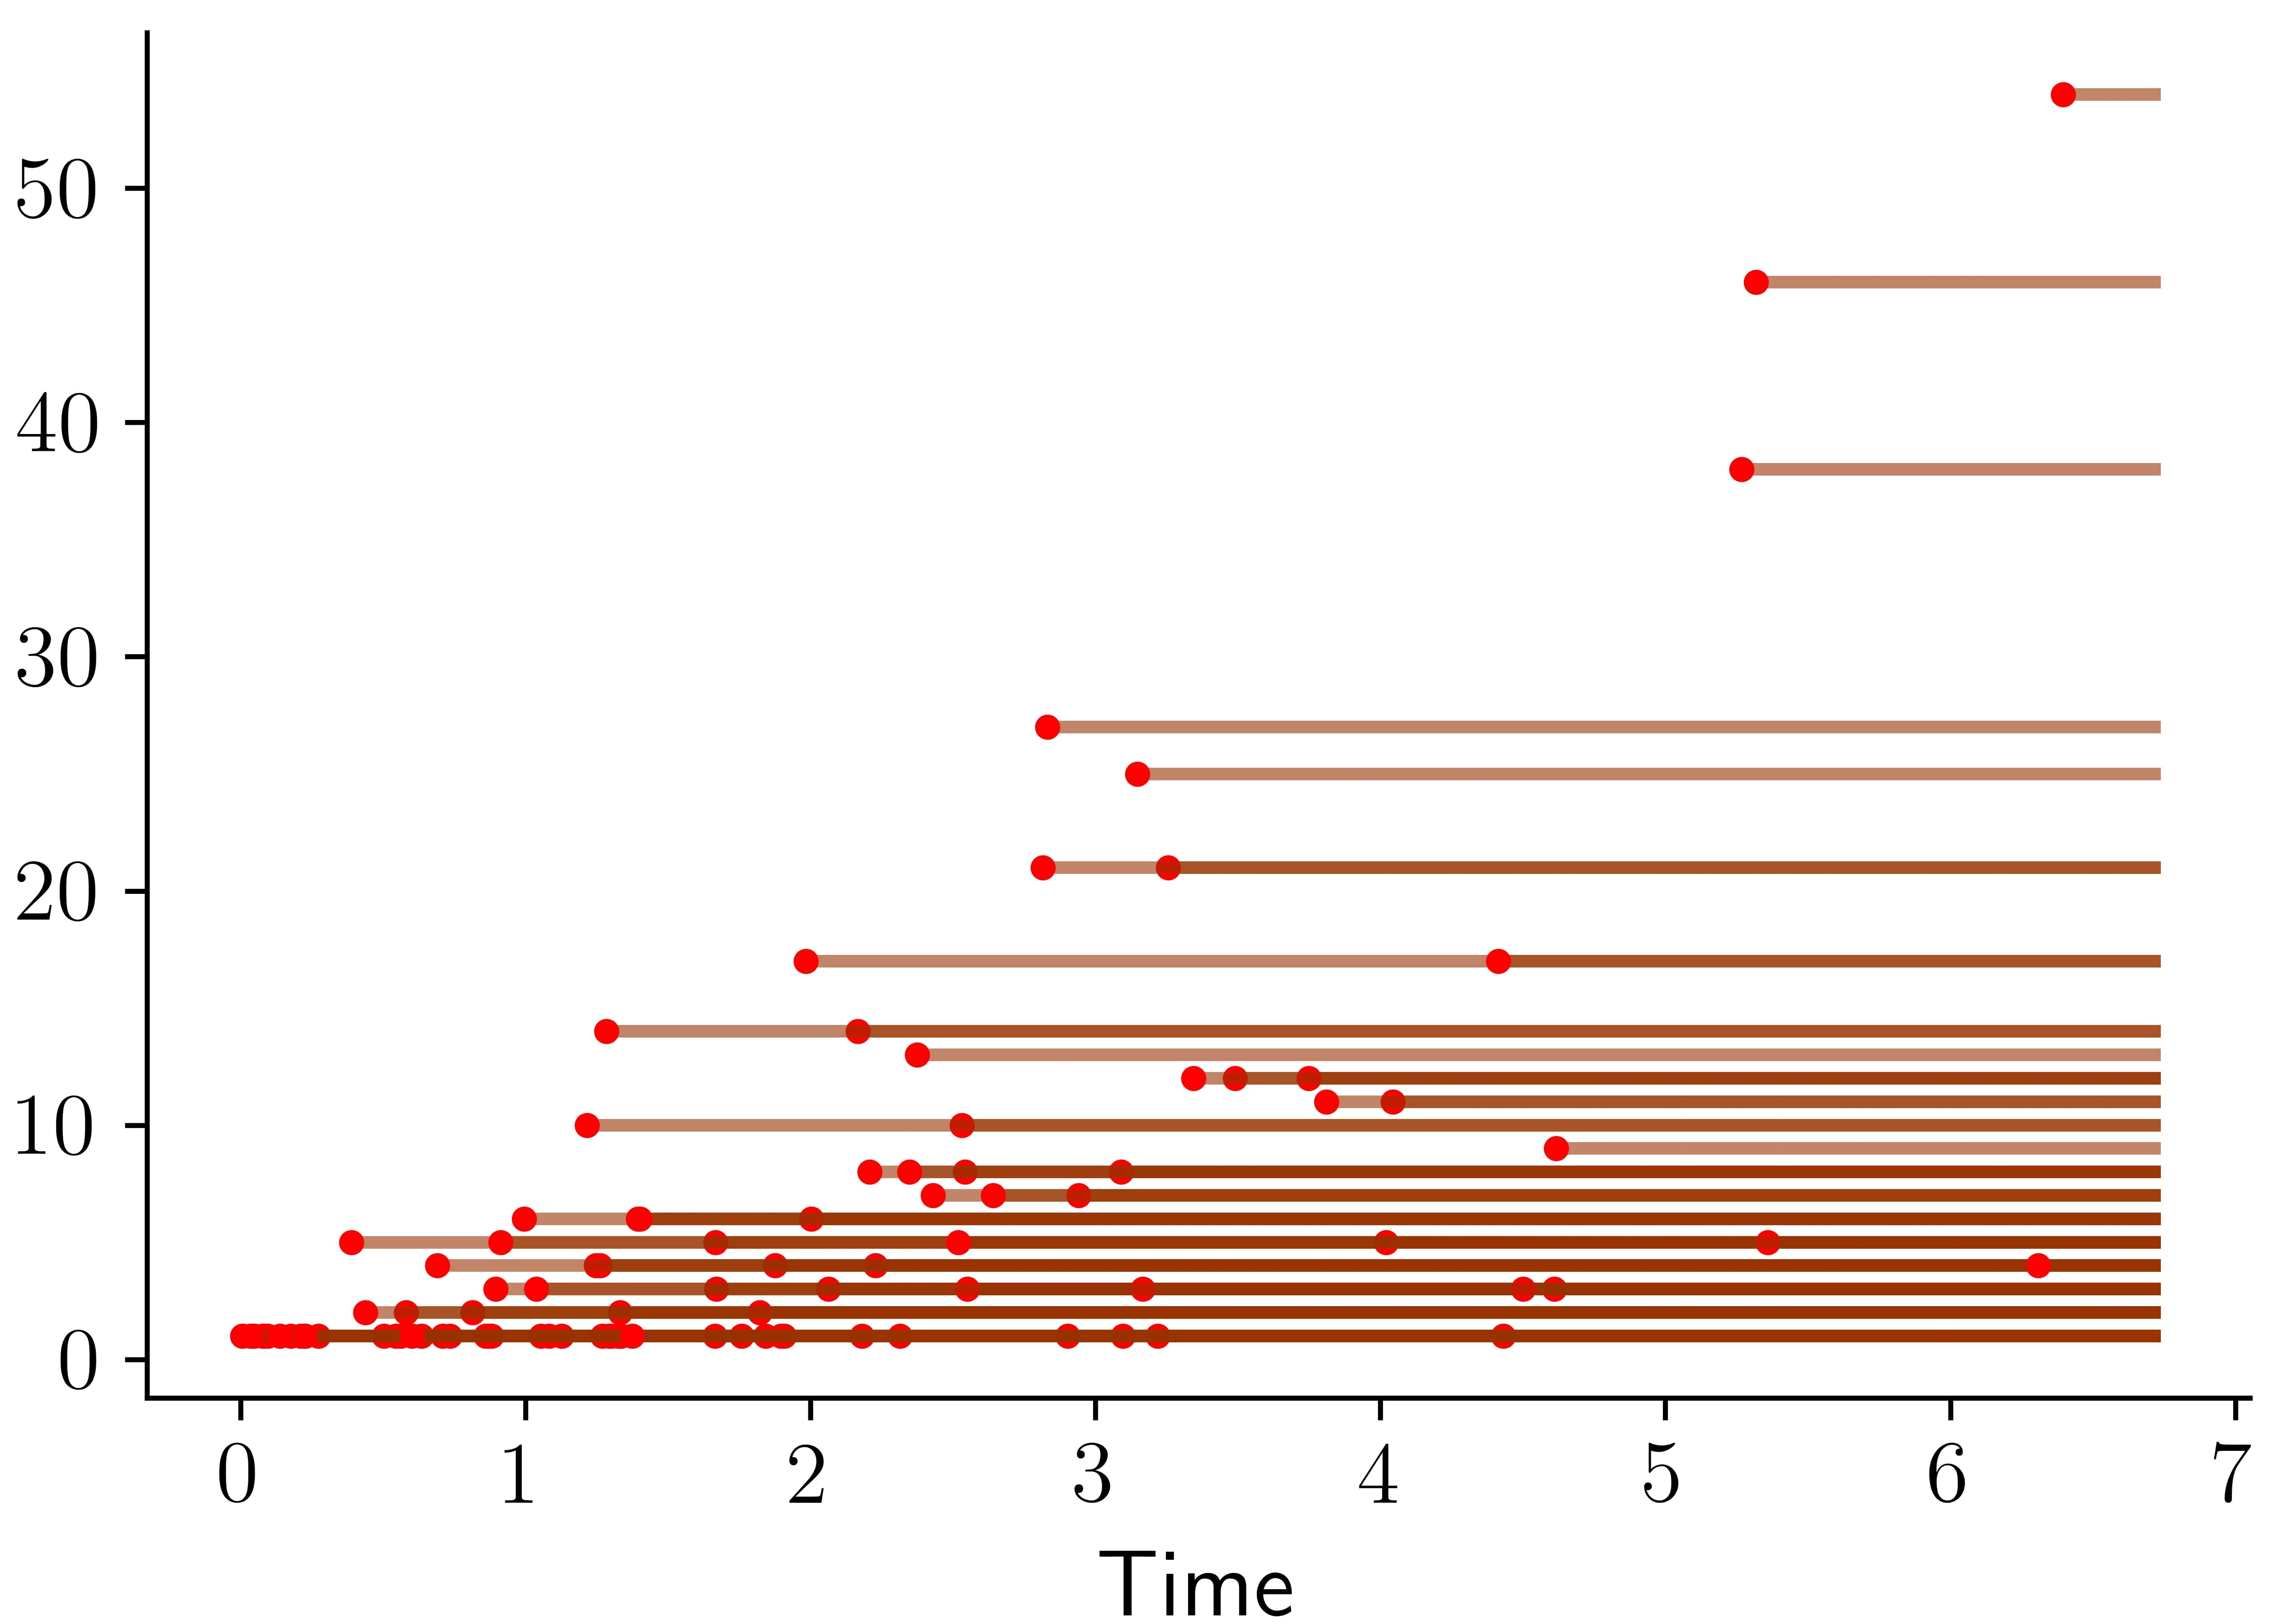
\includegraphics[width = 0.55\textwidth]{figures/IMG_ch4/BDRsimulationsY2.jpg}
\caption{100 realisations of $\wt$ generated using the Gillespie algorithm. $\beta = 1$, $\mu = 0$, $\delta = 0.1$. }
\label{BDRsims}
\end{figure}



%%%%%%%%%%%%%%%%%%%%%%%%%%%%%%%%%%%%%%%%%%%%%%%%%%%%%%%%%%%%%%%%%%%%%%%%%%%%%%%%%%%%%%%%%%%%%%%%%%%%%%%%%%%
